\documentclass[a4paper]{article}
\usepackage{latexsym,amssymb,amsmath,amsbsy,amsopn,amstext,xcolor,multicol}
\usepackage{ctex,hyperref,graphicx,wrapfig,fancybox,listings}
\usepackage{pgf,pgfarrows,pgfnodes,pgfautomata,pgfheaps,pgfshade}
\lstset{language=c++}
\lstset{extendedchars=false}
\lstset{numbers=left,
numberstyle=\tiny,
keywordstyle=\color{blue!70}, commentstyle=\color{red!50!green!50!blue!50},
frame=shadowbox,
rulesepcolor=\color{red!20!green!20!blue!20},
breaklines=true,
basicstyle=\small}
\graphicspath{{pic/}}
\title{\bf Delaunay triangulation for calculating Euclidean distance MST}
\date{2017.6}
\author{翁家翌~2016011446}
\begin{document}
\kaishu
\ttfamily
\maketitle
\tableofcontents
%\newpage
\section{介绍}
在二维平面上给定n个点,求由这n个点所构成的最小生成树,其中距离定义为欧几里得距离。

通过查阅相关资料,我知道了MST的边集$\subseteq$~Delaunay三角剖分得到的边集,因此求平面欧几里得距离最小生成树等价于求给定点集的三角剖分。

该项目实现了两种计算三角剖分的方法,支持将计算得到的方案以图片形式输出到文件或窗口,同时也支持以数据文本的形式保存到文件,并且支持从文件中读取原始数据并且显示到窗口。
\section{使用方法}
\subsection{编译及运行}
本项目依赖一些第三方库:
\begin{itemize}
	\item Boost
	\item OpenCV
	\item CGAL
\end{itemize}
并且使用 CMake 来进行 Makefile 的生成,可以在进入 src 目录后运行如下代码进行编译
\begin{lstlisting}{language=bash}
cd build
cmake ..
make
\end{lstlisting}
编译完成后使用 ./main 来运行程序,或可以使用 ./main -h 来查看帮助。

如果想要生成新的测试数据,点数为100,并且在窗口中显示图像信息,可以运行如下命令:
\begin{lstlisting}{language=bash}
./main -n 100 -w
\end{lstlisting}

如果要测试文件testcase/circle\_100000下的数据,可以运行如下命令:
\begin{lstlisting}{language=bash}
./main -t ../../testcase/circle_100000/
\end{lstlisting}

\subsection{具体参数}
\begin{itemize}
	\item [-h] 查看帮助
	\item [-n] 指定生成的点数,默认10000
	\item [-c] 指定生成点集的形状,有正方形(full square)和圆形(full circle)两个方法,默认为full square
	\item [-t] 测试模式,指定读取文件的目录,默认为../../testcase/test/
	\item [-r] 点坐标生成范围,默认为$[0,10000)$
	\item [-d] 点与点之间的最小间隔,默认为0.001
	\item [-i] 图片的大小,默认为$2000\times 2000$
	\item [-s] 图片的后缀,默认为png
	\item [-w] 在运行窗口中显示图片
	\item [-v] 输出Voronoi图的文本信息
\end{itemize}
\section{运行流程}
\begin{enumerate}
	\item 处理命令行的 command
	\item 生成点集数据 or 从已经存在的 data.txt 中读取点集数据
	\item 计算 Delaunay 三角剖分
	\item 计算 MST
	\item 检验步骤3和4 
	\item 将结果可视化 
\end{enumerate}
\section{系统结构}
\subsection{conf}
该文件被所有文件所包含,其中的内容包括Simple\_point、Edge两个类。

\subsubsection{Simple\_Point}

由于我在 CGAL 的手册中找不到关于修改 Point\_2D 类中 x、y 坐标的方法(read-only),因此放弃继承,自己写一个名为 Simple\_Point 的类,实现平面上二维点坐标运算的一些基本功能。

\subsubsection{Edge}

包含三个基本元素:两个端点的编号以及边权。

允许排序,关键字为边权大小。

\subsection{union\_find\_set}

该文件被 \emph{minimum\_spanning\_tree} 和 \emph{validate} 所包含

\subsubsection{功能}

带路经压缩的并查集。

\subsubsection{接口}

\begin{lstlisting}
bool Is_linked(int x, int y); //x和y是否相连
void Link(int x, int y); //连接x和y
\end{lstlisting}

\subsection{generator}
\subsubsection{功能}
给定 n,生成大小为 n 的点集,其中每个点之间最小间距可通过设置。

支持生成两种数据:正方形与圆形。
\subsubsection{接口}
\begin{lstlisting}
Generator(); //构造函数,调用即可生成在该环境变量下的点集
std::vector<Simple_Point> Save(const std::string &filename);
    //将生成的点集信息存入给定的文件名中,并且返回生成点集列表
\end{lstlisting}
\subsubsection{例子}
\begin{lstlisting}
std::vector<Simple_Point> raw_data;
raw_data = Generator().Save(POINTS_FILENAME);	
\end{lstlisting}
\subsection{delaunay}
\subsubsection{功能}
使用 CGAL 计算 Delaunay Triangulation 和 Voronoi Diagram
\subsubsection{接口}
\begin{lstlisting}
Delaunay_Triangulation(const std::vector<Simple_Point> &raw_data);//构造函数,调用即可生成由该点集所构成的三角剖分
void Save(const std::string triangulation_filename,
          const std::string voronoi_filename,
          std::vector<Edge> &triangulation_data,
          std::vector<std::pair<Simple_Point, Simple_Point> > &voronoi_data);//将生成的三角剖分信息存入给定的文件名中,并且将计算得到的数据存储于后两个参数中
\end{lstlisting}
\subsubsection{蜜汁bug}
生成 Voronoi.png 的时候可能会有一些奇怪的水平/垂直线条,不知道如何完全消除(已经采取了一些措施降低生成这种线条的概率)。
\subsubsection{例子}
\begin{lstlisting}
Delaunay_Triangulation cgal_dt(raw_data);
cgal_dt.Save(TRIANGULATION_FILENAME, VORONOI_FILENAME, triangulation_data, voronoi_data);
\end{lstlisting}
\subsection{minimum\_spanning\_tree}
\subsubsection{功能}
包含求 MST 的两种方法:Kruskal 和 Prim,分别在类 MST 和类 Prim 中实现。
\subsubsection{接口}
\begin{lstlisting}
MST(const std::vector<Edge> &_edge); //MST的构造函数,给定不同的边集信息,用Kruskal计算MST
std::vector<Edge> Save(const std::string &filename); //将Kruskal计算出的MST信息写入文件中并返回该列表,以点编号形式存储
Prim(std::vector<Simple_Point>data); //Prim的构造函数,给定点集信息,用Prim计算MST,点数上限20000
\end{lstlisting}
\subsubsection{例子}
\begin{lstlisting}
MST mymst(triangulation_data);
mst_data = mymst.Save(MST_FILENAME);
Prim prim(raw_data);
\end{lstlisting}
\subsection{validate}
\subsubsection{功能}
自己写的 Delaunay 三角剖分方法,使用分治法,用 DECL 存储边的信息。用于检验三角剖分、MST的正确性。

辅助类:Point3,实现了对三维点坐标的一些基本操作。
\subsubsection{接口}
\begin{lstlisting}
My_Delaunay(std::vector<Simple_Point>data); //构造函数,给定点集信息,计算三角剖分信息和MST
\end{lstlisting}
\subsubsection{例子}
\begin{lstlisting}
My_Delaunay myd(raw_data);
\end{lstlisting}
\subsection{visualization}
使用 OpenCV。(在我都写完代码之后才发现 CGAL 有可视化 Voronoi 图的功能,但是还是觉得OpenCV更好用)
\subsubsection{功能}
将点集、三角剖分、Voronoi 图、二者结合的图和MST图(共5张)可视化,点集上限9999(太多点的可视化效果不好),图片大小上限5000(太大没必要)。
\subsubsection{接口}
\begin{lstlisting}
Visualization(int show_case,
              const std::string &prefix,
              const std::string &suffix,
              const std::vector<Simple_Point> &raw_data,
              const std::vector<Edge> &triangulation_data,
              const std::vector<std::pair<Simple_Point, Simple_Point> > &voronoi_data,
              const std::vector<Edge> &mst_data);
//构造函数,给定文件前缀后缀和之前计算出的数据,存储图像信息
\end{lstlisting}
\subsubsection{例子}
\begin{lstlisting}
Visualization visual(1, PREFIX, SUFFIX, raw_data, triangulation_data, voronoi_data, mst_data);
\end{lstlisting}
\section{性能测试}
设置了最多不能超过五百万个点。

\subsection{可视化效果}
以下是一张500个点的 Voronoi 图可视化之后的效果:\\
\begin{center}
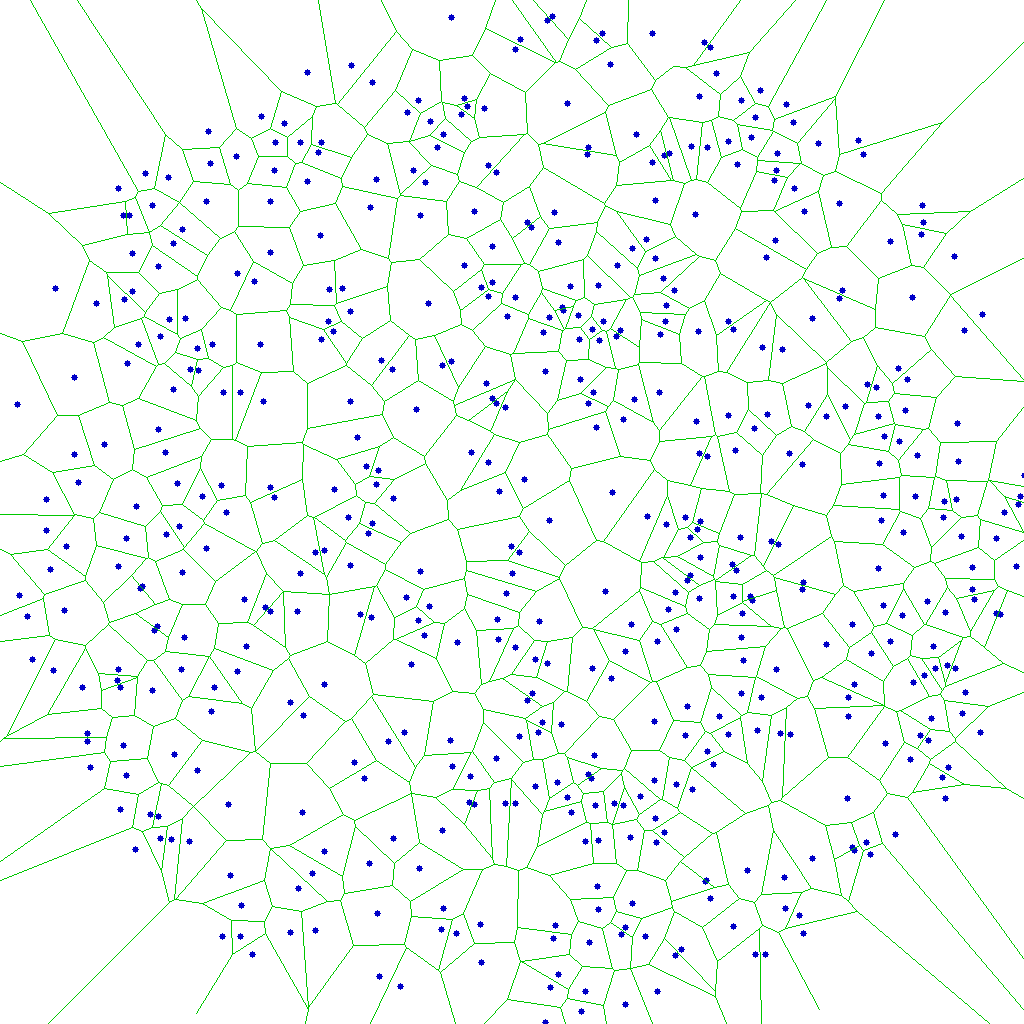
\includegraphics[width=1\linewidth]{../testcase/circle_500/voronoi.png}	
\end{center}

\subsection{运行时间}
以下是运行时间与点集大小的表格:
\begin{center}
\begin{tabular}{lp{2.1cm}p{2cm}p{1.8cm}p{2.25cm}}
\hline
    点集大小 & CGAL增量法三角剖分/ms & 分治法三角剖分/ms & 剖分图上Kruskal/ms & 直接Prim/ms \\\hline
     100 &          0.102 &      0.133 &          0.020 &     0.065 \\
     500 &          0.447 &      1.046 &          0.059 &     1.220 \\
    1000 &          1.155 &      1.538 &          0.123 &     4.570 \\
    3000 &          2.736 &      5.607 &          0.515 &    37.949 \\
    5000 &          3.963 &      9.702 &          0.710 &    99.299 \\
   10000 &         12.926 &     24.061 &          1.316 &   374.725 \\
   20000 &         17.478 &     46.356 &          2.786 &  1510.781 \\
   50000 &         47.449 &    128.215 &          7.601 &         / \\
  100000 &        101.048 &    279.464 &         19.885 &         / \\
  200000 &        203.102 &    577.641 &         48.389 &         / \\
  400000 &        415.429 &   1296.535 &        105.245 &         / \\
  800000 &        894.641 &   2940.455 &        235.292 &         / \\
 1000000 &       1313.407 &   3575.548 &        298.665 &         / \\
\hline
\end{tabular}
\end{center}

以下是表格所对应的数据:\\
\begin{center}
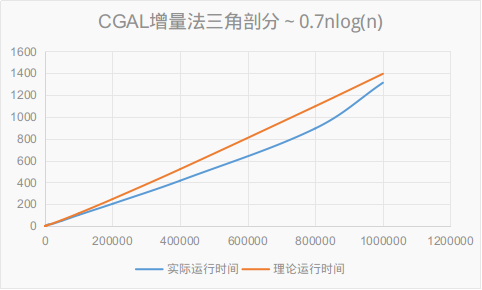
\includegraphics[width=0.9\linewidth]{runtime1.png}

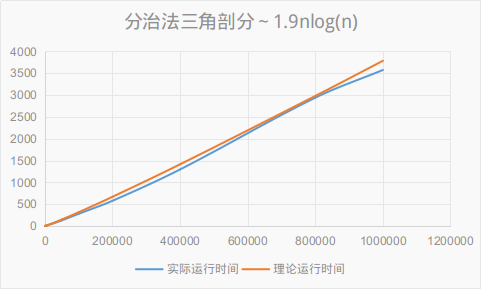
\includegraphics[width=0.9\linewidth]{runtime2.png}

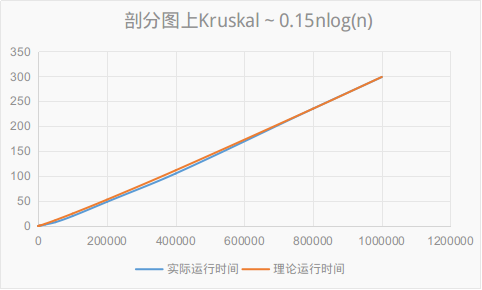
\includegraphics[width=0.9\linewidth]{runtime3.png}

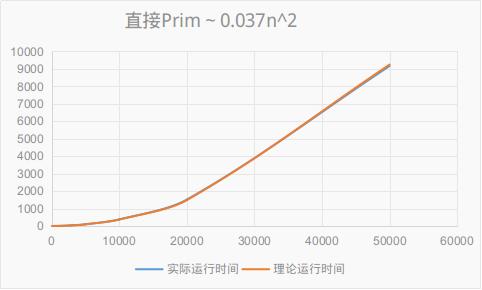
\includegraphics[width=0.9\linewidth]{runtime4.png}	
\end{center}
可以看到,在数据量较大的情况下,Prim算法效率极低,是由于自身的复杂度 $O(n^2)$ 所限制;对于三角剖分,增量法和分治法的效率都趋近于 $O(n\log n)$,但是分治法的效率大约是增量法的三倍。

\subsection{屏幕截图}
以下是实际运行过程中的屏幕截图:
\begin{center}
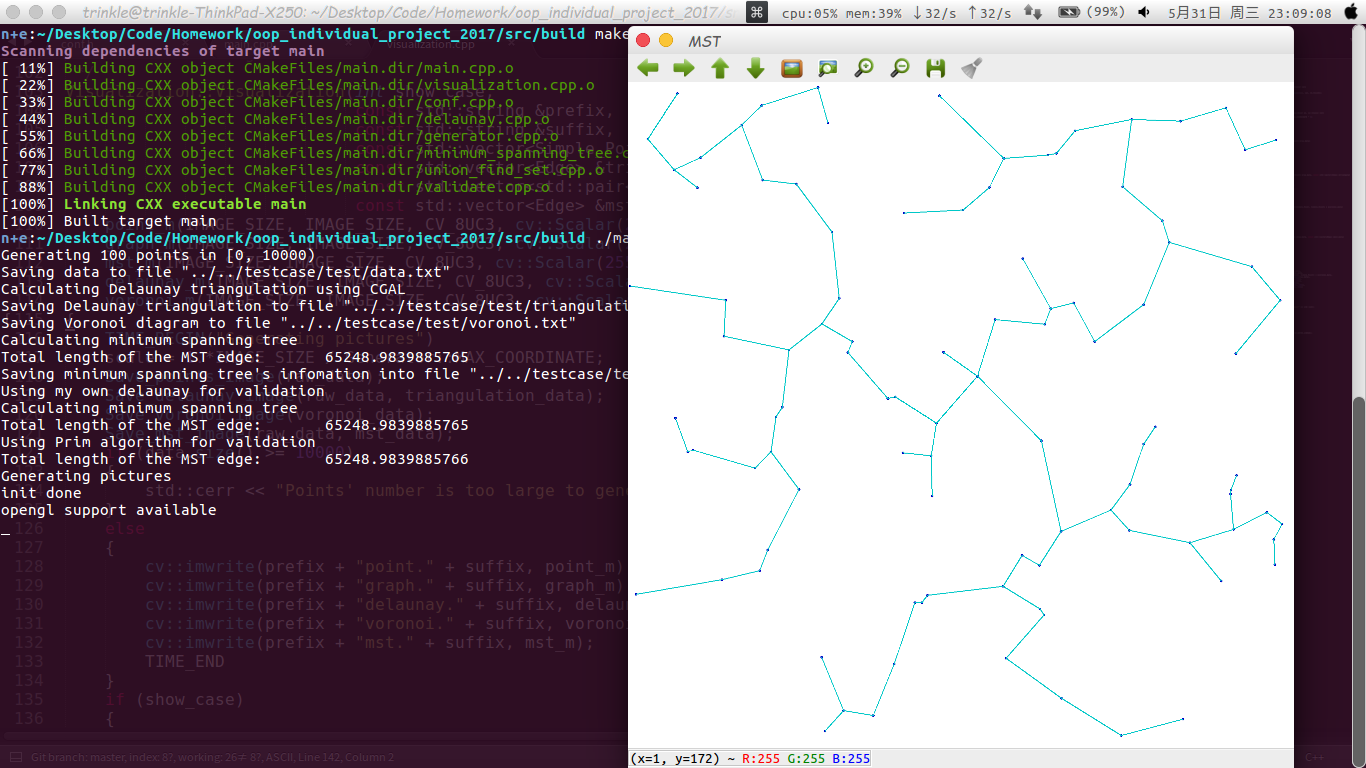
\includegraphics[width=0.9\linewidth]{screen1.png}

~\\

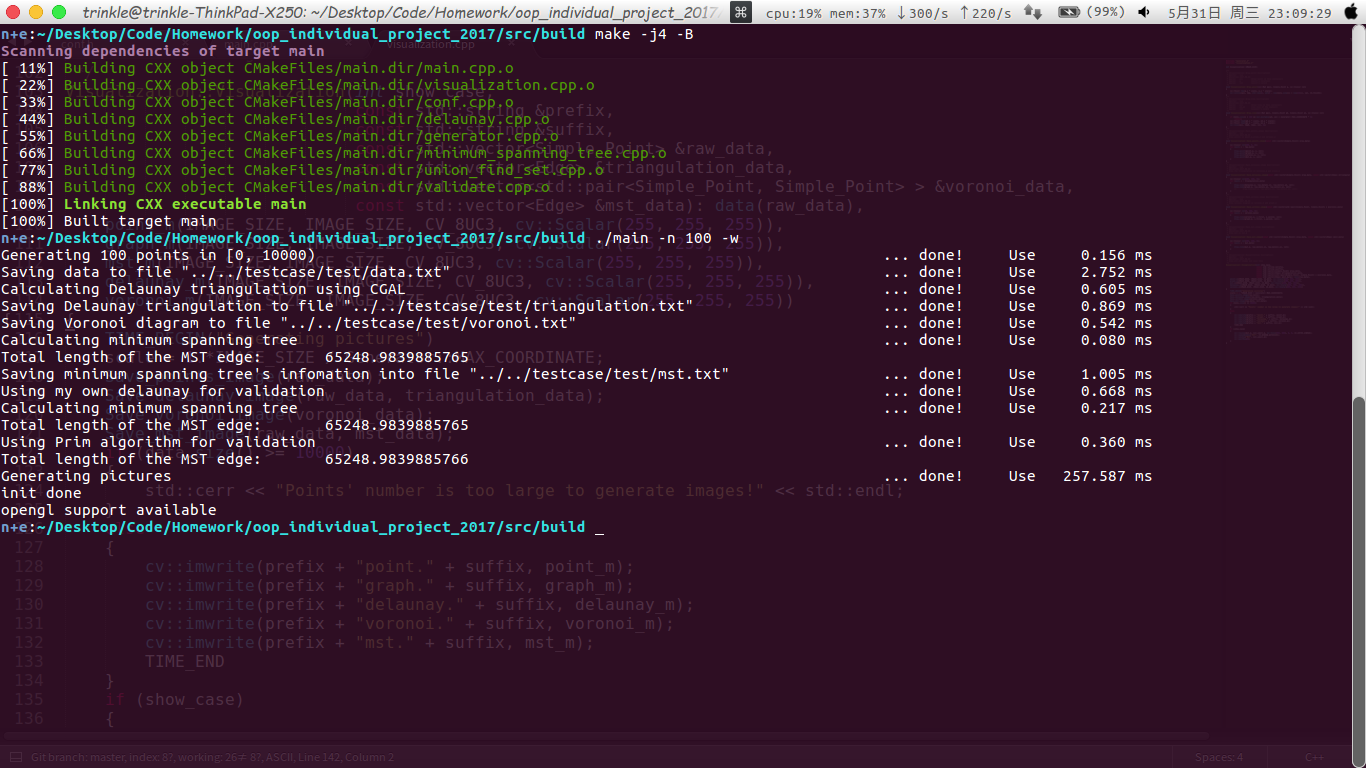
\includegraphics[width=0.9\linewidth]{screen2.png}
\end{center}


\end{document}
